%% generato automaticamente da tools/build_tex.py --- non modificare
\chapter{Una regolarità che dura quattro passi}
\label{cap:factor}
\quaderno{factor.dfw}{18 Aug 2010}{36}

Agosto 2010. Il quaderno insegue un'uguaglianza fra due prodotti di fattoriali, la trova vera nei primi quattro casi, e poi la vede rompersi. Invece di abbandonarla, misura di quanto si rompe: le espressioni successive sono le fattorizzazioni complete delle differenze, numeri di trenta e più cifre scomposti nei loro fattori primi. È l'esempio migliore, in tutta la raccolta, di che cosa un sistema di calcolo simbolico permetta di fare che a mano sarebbe impensabile.

\section{Dove l'uguaglianza vale}

L'affermazione da mettere alla prova è che il prodotto dei fattoriali dei primi numeri dispari sia il fattoriale di un numero triangolare:
\[
  \prod_{n=0}^{p}(2n+1)!\;\overset{?}{=}\;\left(\frac{(p+1)(p+2)}{2}\right)!
\]
Le prime righe scrivono le differenze e le trovano nulle.

\begin{espr}{1}{User}{\verificata}
\[
1! - 1! = 0
\]
\end{espr}
Il caso $p=0$: entrambi i membri valgono $1$.

\begin{espr}{2}{User}{\verificata}
\[
1! \cdot 3! - 3! = 0
\]
\end{espr}
Il caso $p=1$: $1!\cdot3!=6=3!$.

\begin{espr}{3}{User}{\verificata}
\[
1! \cdot 3!\, 5! - 6! = 0
\]
\end{espr}
Il caso $p=2$: $720=6!$.

\begin{espr}{4}{User}{\verificata}
\[
1! \cdot 3!\, 5!\, 7! - 10! = 0
\]
\end{espr}
Il caso $p=3$: $3\,628\,800=10!$. Quattro coincidenze consecutive.


Quattro casi consecutivi, e tutti tornano: $1!=1!$, poi $1!\cdot3!=6=3!$, poi $1!\cdot3!\cdot5!=720=6!$, e infine $1!\cdot3!\cdot5!\cdot7!=3\,628\,800=10!$. I numeri $1,3,6,10$ sono i primi quattro numeri triangolari, e a questo punto una congettura è del tutto ragionevole.

\section{Dove si rompe, e di quanto}

Al quinto passo l'uguaglianza cede. Le righe seguenti non si limitano a constatarlo: fattorizzano la differenza, un caso dopo l'altro, per sei passi.

\begin{espr}{5}{User}{}
\[
1! \cdot 3!\, 5!\, 7!\, 9! - 15! = 2^{11} \cdot 3^{6}\, 5^{3}\, 7^{3}
\]
\end{espr}
Il primo caso in cui l'uguaglianza fallisce. Qui però c'è un refuso: la differenza vale $2^{11}\cdot3^{6}\cdot5^{3}\cdot7^{2}=9\,144\,576\,000$, mentre la riga scrive $7^{3}$. Il valore scritto è dunque sette volte quello vero. Tutte le fattorizzazioni successive, che sono uscite da Derive e non battute a mano, sono invece esatte.

\begin{espr}{6}{User}{\verificata}
\[
1! \cdot 3!\, 5!\, 7!\, 9!\, 11! - 21! = 2^{18} \cdot 3^{9}\, 5^{4}\, 7^{3}\, 11^{3}
\]
\end{espr}
Il caso $p=5$: la differenza contiene $11^3$.

\begin{espr}{7}{User}{\verificata}
\[
1! \cdot 3!\, 5!\, 7!\, 9!\, 11!\, 13! - 28! = 2^{25} \cdot 3^{13}\, 5^{6}\, 7^{4}\, 11^{2}\, 13\, 7103
\]
\end{espr}
Il caso $p=6$: compare il primo fattore primo estraneo ai fattoriali, $7103$.

\begin{espr}{8}{User}{\verificata}
\[
1! \cdot 3!\, 5!\, 7!\, 9!\, 11!\, 13!\, 15! - 36! = 2^{34} \cdot 3^{17}\, 5^{8}\, 7^{5}\, 11^{3}\, 13^{2}\, 4013\, 4261
\]
\end{espr}
Il caso $p=7$: due fattori primi a quattro cifre, $4013$ e $4261$.

\begin{espr}{9}{User}{\verificata}
\[
1! \cdot 3!\, 5!\, 7!\, 9!\, 11!\, 13!\, 15!\, 17! - 45! = 2^{41} \cdot 3^{21}\, 5^{10}\, 7^{6}\, 11^{5}\, 13^{3}\, 17\, 8933\, 22969787
\]
\end{espr}
Il caso $p=8$: compare $22\,969\,787$.

\begin{espr}{10}{User}{\verificata}
\begin{align*}
& 1! \cdot 3!\, 5!\, 7!\, 9!\, 11!\, 13!\, 15!\, 17!\, 19! - 55! \\
=\;& 2^{50} \cdot 3^{26}\, 5^{13}\, 7^{8}\, 11^{6}\, 13^{4}\, 17^{2}\, 19\, 3116563\, 333915299
\end{align*}
\end{espr}
Il caso $p=9$: compaiono $3\,116\,563$ e $333\,915\,299$. Nessuno di questi ha rapporto con i fattoriali di partenza.

\begin{espr}{11}{Fctr(User)}{}
\[
2^{64} \cdot 3^{31}\, 5^{15}\, 7^{10}\, 11^{6}\, 13^{7}\, 17^{3}\, 19^{2}\, 251\, 6184811\, 13366363319
\]
\end{espr}
Il caso $p=10$, dato solo nella forma fattorizzata.

\begin{espr}{12}{Fctr(User)}{}
\[
2^{74} \cdot 3^{36}\, 5^{18}\, 7^{12}\, 11^{7}\, 13^{7}\, 17^{4}\, 19^{3}\, 23\, 1543\, 3529737954001890223489333
\]
\end{espr}
Il caso $p=11$: l'ultimo fattore ha venticinque cifre.

\begin{espr}{13}{Fctr(User)}{}
\[
2^{86} \cdot 3^{44}\, 5^{21}\, 7^{14}\, 11^{8}\, 13^{7}\, 17^{5}\, 19^{4}\, 23^{2}\, 7527420903061154660844431547708509201
\]
\end{espr}
Il caso $p=12$: la parte non piccola è un unico numero di trentasette cifre.

\begin{espr}{14}{Fctr(User)}{}
\[
2^{101} \cdot 3^{50}\, 5^{25}\, 7^{17}\, 11^{9}\, 13^{8}\, 17^{6}\, 19^{5}\, 23^{3}\, 267661\, 669113\, 96487944706595864404794370019938759
\]
\end{espr}
Il caso $p=13$.

\begin{espr}{15}{Fctr(User)}{}
\[
2^{116} \cdot 3^{58}\, 5^{28}\, 7^{19}\, 11^{10}\, 13^{9}\, 17^{7}\, 19^{6}\, 23^{4}\, 29\, 967\, 106487\, 459130657\, 3283850683\, 26841959932382587431547457373253
\]
\end{espr}
Il caso $p=14$: la differenza contiene un fattore primo di trentadue cifre.


La rottura è netta ma non catastrofica. Al primo caso in cui fallisce, $p=4$, la differenza vale poco più di nove miliardi contro un valore comune di circa $1{,}3\cdot10^{12}$: uno scarto dello $0{,}7\%$. Ai passi successivi la differenza cresce molto più in fretta dei due prodotti, e già a $p=9$ nella sua fattorizzazione compaiono primi enormi — $3\,116\,563$ e $333\,915\,299$ — che non hanno nulla a che vedere con i piccoli fattori dei fattoriali.

È questo il segnale che la congettura non era vicina al vero ma solo fortunata all'inizio. Se la differenza fosse un errore sistematico piccolo, i suoi fattori resterebbero fra i primi che compongono i fattoriali; il fatto che compaiano fattori primi grandi e apparentemente casuali dice che i due numeri non hanno alcuna relazione aritmetica al di là della coincidenza iniziale.

\section{L'enunciato generale e i casi verificati}

Una riga sola scrive la differenza in forma generale, e le quattro seguenti riverificano i casi che funzionano mostrando anche le fattorizzazioni dei due membri.

\begin{espr}{16}{User}{}
\[
\prod_{n=0}^{p} \left(2\, n + 1\right)! - \left(\frac{\left(p + 1\right)\, \left(p + 2\right)}{2}\right)!
\]
\end{espr}
L'enunciato generale della differenza, che è ciò che tutte le righe precedenti hanno valutato.

\begin{figure}[htbp]
  \centering
  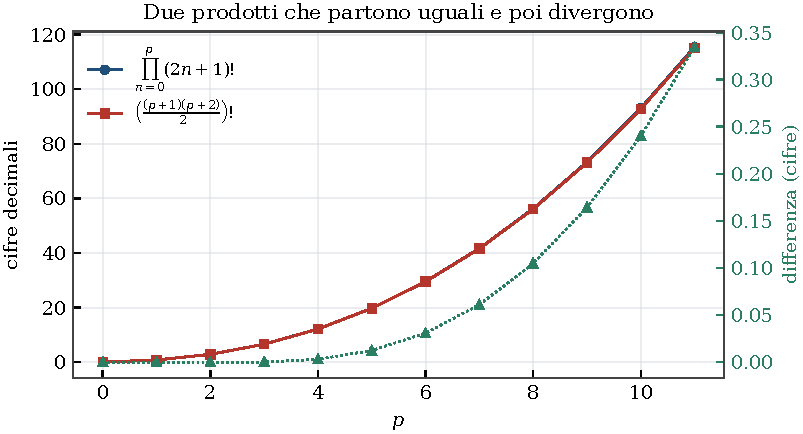
\includegraphics[width=0.86\linewidth]{../figures/factor.pdf}
  \caption{I due membri dell'uguaglianza, misurati in numero di cifre decimali. Coincidono fino a $p=3$ e poi si separano; la curva tratteggiata sull'asse destro è la loro differenza, che cresce senza limite.}
  \label{fig:factor}
\end{figure}
\begin{espr}{17}{User}{\verificata}
\[
1! = 1 = 1!
\]
\end{espr}
La verifica del caso $p=0$, con entrambi i membri.

\begin{espr}{18}{User}{\verificata}
\[
1! \cdot 3! = 2 \cdot 3 = 3!
\]
\end{espr}
Il caso $p=1$, con la fattorizzazione $2\cdot3$.

\begin{espr}{19}{User}{\verificata}
\[
1! \cdot 3!\, 5! = 2^{4} \cdot 3^{2}\, 5 = 6!
\]
\end{espr}
Il caso $p=2$: $2^4\cdot3^2\cdot5=6!$.

\begin{espr}{20}{User}{\verificata}
\[
1! \cdot 3!\, 5!\, 7! = 2^{8} \cdot 3^{4}\, 5^{2}\, 7 = 10!
\]
\end{espr}
Il caso $p=3$: $2^8\cdot3^4\cdot5^2\cdot7=10!$. È l'ultimo che funziona.


Le righe $\#17$--$\#20$ sono la stessa verifica dei primi quattro casi, ma questa volta con i due membri scritti nella loro forma fattorizzata: $2^4\cdot3^2\cdot5=720=6!$ e $2^8\cdot3^4\cdot5^2\cdot7=3\,628\,800=10!$. Serve a vedere che gli esponenti combaciano — che è il modo naturale di controllare un'uguaglianza fra prodotti di fattoriali.

\section{Le fattorizzazioni dei fattoriali triangolari}

L'ultima sezione fattorizza il secondo membro per i valori successivi, cioè i fattoriali $15!$, $21!$, $28!$, $36!$, $45!$, $55!$, $66!$, $78!$.

\begin{espr}{21}{User}{}
\[
15!
\]
\end{espr}
Il primo fattoriale triangolare per cui l'uguaglianza fallisce.

\begin{espr}{22}{Fctr(\#21)}{}
\[
2^{11} \cdot 3^{6}\, 5^{3}\, 7^{2}\, 11\, 13
\]
\end{espr}
La sua fattorizzazione. Da confrontare con la riga $\#5$: gli esponenti di $2$, $3$ e $5$ coincidono, quello di $7$ no, e in più compaiono $11$ e $13$.

\begin{espr}{23}{User}{}
\[
21!
\]
\end{espr}
Il fattoriale successivo.

\begin{espr}{24}{Fctr(\#23)}{}
\[
2^{18} \cdot 3^{9}\, 5^{4}\, 7^{3}\, 11\, 13\, 17\, 19
\]
\end{espr}
La sua fattorizzazione.

\begin{espr}{25}{User}{}
\[
28!
\]
\end{espr}
E il successivo.

\begin{espr}{26}{Fctr(\#25)}{}
\[
2^{25} \cdot 3^{13}\, 5^{6}\, 7^{4}\, 11^{2}\, 13^{2}\, 17\, 19\, 23
\]
\end{espr}
La sua fattorizzazione.

\begin{espr}{27}{User}{}
\[
\left(\frac{\left(7 + 1\right)\, \left(7 + 2\right)}{2}\right)!
\]
\end{espr}
Lo stesso numero scritto con la formula del numero triangolare.

\begin{espr}{28}{Fctr(\#27)}{}
\[
2^{34} \cdot 3^{17}\, 5^{8}\, 7^{5}\, 11^{3}\, 13^{2}\, 17^{2}\, 19\, 23\, 29\, 31
\]
\end{espr}
La sua fattorizzazione: compaiono tutti i primi fino a $31$.

\begin{espr}{29}{Sub(User)}{}
\[
\left(\frac{\left(8 + 1\right)\, \left(8 + 2\right)}{2}\right)!
\]
\end{espr}
Il passo successivo.

\begin{espr}{30}{Fctr(\#29)}{}
\[
2^{41} \cdot 3^{21}\, 5^{10}\, 7^{6}\, 11^{4}\, 13^{3}\, 17^{2}\, 19^{2}\, 23\, 29\, 31\, 37\, 41\, 43
\]
\end{espr}
La fattorizzazione arriva a $43$.

\begin{espr}{31}{Sub(\#16')}{}
\[
\left(\frac{\left(9 + 1\right)\, \left(9 + 2\right)}{2}\right)!
\]
\end{espr}
E ancora.

\begin{espr}{32}{Fctr(\#31)}{}
\[
2^{50} \cdot 3^{26}\, 5^{13}\, 7^{8}\, 11^{5}\, 13^{4}\, 17^{3}\, 19^{2}\, 23^{2}\, 29\, 31\, 37\, 41\, 43\, 47\, 53
\]
\end{espr}
Fino a $53$.

\begin{espr}{33}{Sub(\#16')}{}
\[
\left(\frac{\left(10 + 1\right)\, \left(10 + 2\right)}{2}\right)!
\]
\end{espr}
Il numero triangolare di indice dieci.

\begin{espr}{34}{Fctr(\#33)}{}
\[
2^{64} \cdot 3^{31}\, 5^{15}\, 7^{10}\, 11^{6}\, 13^{5}\, 17^{3}\, 19^{3}\, 23^{2}\, 29^{2}\, 31^{2}\, 37\, 41\, 43\, 47\, 53\, 59\, 61
\]
\end{espr}
La fattorizzazione arriva a $61$.

\begin{espr}{35}{Sub(\#16')}{}
\[
\left(\frac{\left(11 + 1\right)\, \left(11 + 2\right)}{2}\right)!
\]
\end{espr}
Quello di indice undici.

\begin{espr}{36}{Fctr(\#35)}{}
\[
2^{74} \cdot 3^{36}\, 5^{18}\, 7^{12}\, 11^{7}\, 13^{6}\, 17^{4}\, 19^{4}\, 23^{3}\, 29^{2}\, 31^{2}\, 37^{2}\, 41\, 43\, 47\, 53\, 59\, 61\, 67\, 71\, 73
\]
\end{espr}
L'ultima fattorizzazione del quaderno: tutti i primi fino a $73$, con gli esponenti dati dalla formula di Legendre.


Il confronto con le fattorizzazioni delle differenze della prima sezione è istruttivo. I fattoriali contengono tutti i primi fino al loro argomento, con esponenti che seguono la formula di Legendre; le differenze contengono invece pochi primi piccoli con esponenti alti e poi qualche primo grande isolato. Le due strutture non si assomigliano, e questo è, in sostanza, la risposta alla domanda che il quaderno si era posto.

\section*{In sintesi}
\addcontentsline{toc}{section}{In sintesi}

Un'uguaglianza vera quattro volte di seguito e poi falsa per sempre è un buon promemoria sul valore delle verifiche numeriche. Il quaderno lo raccoglie nel modo giusto: non si limita a constatare il fallimento ma lo quantifica, e la struttura dei fattori primi delle differenze dice, meglio di qualunque argomento, che la coincidenza iniziale non nascondeva nulla.

Da segnalare che l'unica riga battuta a mano di tutta la sezione — la $\#5$ — contiene un errore di trascrizione nell'esponente di $7$, mentre tutte le fattorizzazioni prodotte da Derive sono esatte. È il secondo refuso della raccolta, dopo quello di \dfw{teoria.dfw} (capitolo~\ref{cap:teoria}), e come quello sta in una riga scritta dall'autore.

